% Chapter 8
\chapter{CONCLUSIONS} % Write in your own chapter title
\section{Conclusion}
A working model of Automatic vehicle accident detection and messaging system using a GPS and GSM modems has been implemented successfully. The biggest advantage of our project is, whenever the sensor is activated we will be immediately getting the acknowledgement from GSM modem to our mobile number. This system locates the accident spot accurately, realizing the automation of accident detection and messaging system. Consequently, it will save the precious time required to save the accident victims. Further this system can be implemented using the vibration sensors as well as the sound sensors, in order to make it more accurate and efficient to detect an accident

\section{Future Work}

The data stored at the remote server is so far unused. There can be new information which can be derived from analysing this data. This information can be useful to the public and the government in creating new and proper traffic rules and restrictions. There are different ways of analysing data.Some ways are briefly described here.

\subsection{Time series}
A single variable is captured over a period of time, such as the no.of accidents over a 10-year period. A line chart may be used to demonstrate the trend. This is shown in Figure \ref{fig:time}

\begin{figure}[h!]
	\centering
	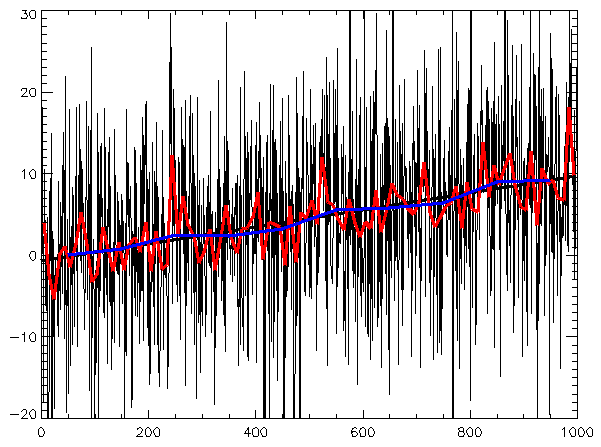
\includegraphics[scale=0.3]{time}
	\caption{Time series}
	\label{fig:time}
\end{figure}

\subsection{Correlation}
Comparison between observations represented by two variables (X,Y) to determine if they tend to move in the same or opposite directions. For example, plotting unemployment (X) and inflation (Y) for a sample of months. A scatter plot as shown in Figure \ref{fig:scatter} is typically used for this message.

\begin{figure}[h!]
	\centering
	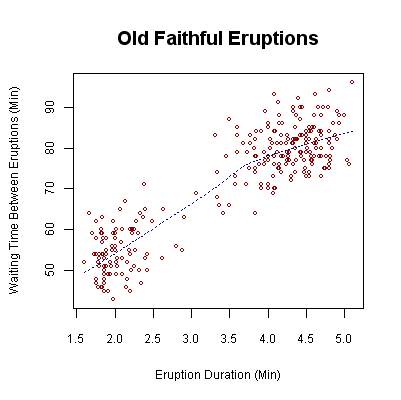
\includegraphics[scale=0.4]{scatter}
	\caption{Scatter plot}
	\label{fig:scatter}
\end{figure}

\newpage
\subsection{Analytical Activities of the Data Users}
Users may have particular data points of interest within a data set, such low-level user analytic activities are given below

\begin{table}[!ht]
	\centering
	\begin{tabular}{| m{4em} | m{6em}| m{7em} | m{8em} |} 
		\hline
		\textbf{Task} & \textbf{General description} & \textbf{Abstract} & \textbf{Examples} \\ 
		\hline
		Retrieve value & Find attributes from a set & What are values of attributes in data cases & Name of victim\\ 
		\hline
		Compute derived values & Compute an aggregate numeric representation & What is value of aggregate function F over a set S of cases? & What is the average number of accidents ? \\ 
		\hline
		Find extremum & Find extreme values in data cases & What are the top/bottom data w.r.t attribute A? & Type of vehicles involved in frequent accidents \\
		\hline
		Sort & Given a set of data cases, rank them according to some ordinal metric & What is the sorted order of a set S of data cases according to value of attribute A? & Order accident based on time \\
		\hline
	\end{tabular}
	\caption{Types of analytics}
\end{table}

Apart from the data analysis, the scope of the proposed work can be extended to include \\
\begin{itemize}
	\item Use in automotives and transport vehicles - from lighter vehicles like cars, to heavier automotives like ships and aeroplanes.
	\item Security and remote monitoring of vehicles especially during military operations. 
	\item Be more interfaced with vehicle airbag system such that when the sensors detect the accident, the air bags get opened
	\item Use for real time monitoring of traffic.
	\item Better methods to help the user in reporting false alarms.
\end{itemize}

